\documentclass[a4paper,11pt]{article}
\usepackage[utf8]{inputenc}
\usepackage[polish]{babel}
\usepackage[T1]{fontenc}
\usepackage{times}
\usepackage{graphicx}
\usepackage{anysize}
\usepackage{amsmath}
\usepackage{color}
\usepackage{listings}
\lstloadlanguages{C}

%\marginsize{left}{right}{top}{bottom}
\marginsize{2.5cm}{2.5cm}{2.5cm}{2.5cm}

\definecolor{darkred}{rgb}{0.9,0,0}
\definecolor{grey}{rgb}{0.4,0.4,0.4}
\definecolor{orange}{rgb}{1,0.6,0.05}
\definecolor{darkgreen}{rgb}{0.2,0.5,0.05}
\lstset{language=C,
	basicstyle=\ttfamily\small,
	keywordstyle=\color{darkgreen}\ttfamily\bfseries\small,
	stringstyle=\color{red}\ttfamily\small,
	commentstyle=\color{grey}\ttfamily\small,
	numbers=left,
	numberstyle=\color{darkred}\ttfamily\scriptsize,
	identifierstyle=\color{blue}\ttfamily\small,
	showstringspaces=false,
	morekeywords={
}}

\begin{document}
\section*{C/Tablice} 
W rozdziale Zmienne w C dowiedziałeś się, jak przechowywać pojedyncze liczby oraz znaki. Czasami zdarza się jednak, że potrzebujemy przechować kilka, kilkanaście albo i więcej zmiennych jednego typu. Nie tworzymy wtedy np. dwudziestu osobnych zmiennych. W takich przypadkach z pomocą przychodzi nam tablica.

Tablica to ciąg zmiennych jednego typu. Ciąg taki posiada jedną nazwę a do jego poszczególnych elementów odnosimy się przez numer (indeks).

\subsection*{Wstęp} 
	\begin{figure}[!htb]
		\centerline{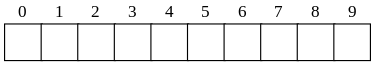
\includegraphics{Array}}
		\caption{Tablica.}
		\label{fig:Talbica dwuwymiarowa}
	\end{figure}
\subsubsection*{Sposoby deklaracji tablic}
Tablicę deklaruje się w następujący sposób:
	


\begin{verbatim}
typ nazwa_tablicy[rozmiar];
\end{verbatim}
gdzie rozmiar oznacza ile zmiennych danego typu możemy zmieścić w tablicy. Zatem aby np. zadeklarować tablicę, mieszczącą 20 liczb całkowitych możemy napisać tak:

\begin{lstlisting}[caption=Deklaracja tablicy, captionpos=b,
label=src:passive2,frame=TB,numbers=none]
int tablica[20];
\end{lstlisting}
Podobnie jak przy deklaracji zmiennych, także tablicy możemy nadać wartości początkowe przy jej deklaracji. Odbywa się to przez umieszczenie wartości kolejnych elementów oddzielonych przecinkami wewnątrz nawiasów klamrowych:
\begin{lstlisting}[caption=Deklaracja tablicy, captionpos=b,
label=src:passive2,frame=TB,numbers=none]
int tablica[3] = {0,1,2};
\end{lstlisting}
Niekoniecznie trzeba podawać rozmiar tablicy, np.:
\begin{lstlisting}[caption=Deklaracja tablicy, captionpos=b,
label=src:passive2,frame=TB,numbers=none]
int tablica[] = {1, 2, 3, 4, 5};
\end{lstlisting}
W takim przypadku kompilator sam ustali rozmiar tablicy (w tym przypadku - 5 elementów).

\noindent
Rozpatrzmy następujący kod:
\begin{lstlisting}[caption=Deklaracja tablicy, captionpos=b,
label=src:passive2,frame=TB,numbers=none]
#include <stdio.h>
#define ROZMIAR 3
int main()
{
	int tab[ROZMIAR] = {3,6,8};
	int i;
	puts ("Druk tablicy tab:");

	for (i=0; i<ROZMIAR; ++i) {
		printf ("Element numer %d = %d\n", i, tab[i]);
	}
	return 0;
}
\end{lstlisting}
Wynik:
\begin{verbatim}
Druk tablicy tab:
Element numer 0 = 3
Element numer 1 = 6
Element numer 2 = 8
\end{verbatim}
Jak widać, wszystko się zgadza.

\noindent
W powyżej zamieszczonym przykładzie użyliśmy stałej do podania rozmiaru tablicy. Jest to o tyle pożądany zwyczaj, że w razie potrzeby zmiany rozmiaru tablicy, zmieniana jest tylko wartość w jednej linijce kodu przy \#define, w innym przypadku musielibyśmy szukać wszystkich wystąpień rozmiaru rozsianych po kodzie całego programu.

\subsection*{Odczyt/zapis wartości do tablicy} 
Tablicami posługujemy się tak samo jak zwykłymi zmiennymi. Różnica polega jedynie na podawaniu indeksu tablicy. Określa on, z którego elementu (wartości) chcemy skorzystać spośród wszystkich umieszczonych w tablicy. Numeracja indeksów rozpoczyna się od zera, co oznacza, że pierwszy element tablicy ma indeks równy 0, drugi 1, trzeci 2, itd.

\noindent
Spróbujmy przedstawić to na działającym przykładzie. Przeanalizuj następujący kod:
\begin{lstlisting}[caption=Odczyt wartości do tablicy, captionpos=b,
label=src:passive2,frame=TB,numbers=none]
int tablica[5] = {0};
int i = 0;
tablica[2] = 3;
tablica[3] = 7;
for (i=0;i!=5;++i) {
printf ("tablica[%d]=%d\n", i, tablica[i]);
}
\end{lstlisting}
Jak widać, na początku deklarujemy 5-elementową tablicę, którą od razu zerujemy. Następnie pod trzeci i czwarty element (liczone począwszy od 0) podstawiamy liczby 3 i 7. Pętla ma za zadanie wyprowadzić wynik naszych działań.

\noindent
Tablica może być również zmieniana w obrębie funkcji.
\subsection*{Tablice znaków} 
Tablice znaków, tj. typu char oraz unsigned char, posiadają dwie ogólnie przyjęte nazwy, zależnie od ich przeznaczenia:
	\begin{itemize}
	
	\item bufory - gdy wykorzystujemy je do przechowywania ogólnie pojętych danych, gdy traktujemy je jako po prostu "ciągi bajtów" (typ char ma rozmiar 1 bajta, więc jest elastyczny do przechowywania np. danych wczytanych z pliku przed ich przetworzeniem).
	\item napisy - gdy zawarte w nich dane traktujemy jako ciągi liter; jest im poświęcony osobny rozdział Napisy.
	\end{itemize}
\noindent
Przykład:
\begin{lstlisting}[caption=Tablice znaków, captionpos=b,
label=src:passive2,frame=TB,numbers=none]
/*
http://joequery.me/code/snprintf-c/


gcc a.c -Wall
./a.out

012345678
hello th\0
turtle\078
2222\05678

*/ 
#include<stdio.h>
#define BUFSIZE 9




void init_buf(char *buf, size_t size){
	int i;
	for(i=0; i<size; i++){
		buf[i] = i + '0'; // int to char conversion
	}
}

void print_buf(char *buf){
	int i;
	char c;
	for(i=0; i<BUFSIZE; i++){
		c = buf[i];
		if(c == '\0'){
			printf("\\0");	
		}
		else{
			printf("%c", buf[i]);
		}
	}
	printf("\n");
}


int main(){
	char buf[BUFSIZE];
	init_buf(buf, BUFSIZE);
	print_buf(buf);
	
	// hello there! == 12 characters, > BUFSIZE
	init_buf(buf, BUFSIZE);
	snprintf(buf, BUFSIZE, "hello there!");
	print_buf(buf);

	// turtle == 6 charaters, < BUFSIZE
	init_buf(buf, BUFSIZE);
	snprintf(buf, BUFSIZE, "turtle");
	print_buf(buf);
	
	// 2222220 == 7 charaters, > 5
	init_buf(buf, BUFSIZE);
	snprintf(buf, 5, "%d", 222222 * 10);
	print_buf(buf);
	
	return 0;
}
\end{lstlisting}

\subsection*{Tablice wielowymiarowe} 
\begin{figure}[!htb]
	\centerline{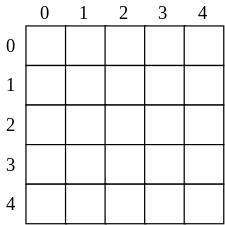
\includegraphics{Array2}}
	\caption{Tablica dwuwymiarowa.}
	\label{fig:Talbica dwuwymiarowa}
\end{figure}

Rozważmy teraz konieczność przechowania w pamięci komputera całej macierzy o wymiarach 10 x 10. Można by tego dokonać tworząc 10 osobnych tablic jednowymiarowych, reprezentujących poszczególne wiersze macierzy. Jednak język C dostarcza nam dużo wygodniejszej metody, która w dodatku jest bardzo łatwa w użyciu. Są to \textbf{tablice wielowymiarowe}, lub inaczej "tablice tablic". Tablice wielowymiarowe definiujemy podając przy zmiennej kilka wymiarów, np.:
\begin{lstlisting}[caption=Tablice wielowymiarowe, captionpos=b,
label=src:passive2,frame=TB,numbers=none]
float macierz[10][10];
\end{lstlisting}
Tak samo wygląda dostęp do poszczególnych elementów tablicy:
\begin{lstlisting}[caption=Tablice wielowymiarowe, captionpos=b,
label=src:passive2,frame=TB,numbers=none]
macierz[2][3] = 1.2;
\end{lstlisting}
Jak widać ten sposób jest dużo wygodniejszy (i zapewne dużo bardziej "naturalny") niż deklarowanie 10 osobnych tablic jednowymiarowych. Aby zainicjować tablicę wielowymiarową należy zastosować zagłębianie klamr, np.:
\begin{lstlisting}[caption=Tablice wielowymiarowe, captionpos=b,
label=src:passive2,frame=TB,numbers=none]
 float macierz[3][4] = {
	{ 1.6, 4.5, 2.4, 5.6 },  /* pierwszy wiersz */
	{ 5.7, 4.3, 3.6, 4.3 },  /* drugi wiersz */
	{ 8.8, 7.5, 4.3, 8.6 }   /* trzeci wiersz */
};
\end{lstlisting}
Dodatkowo, pierwszego wymiaru nie musimy określać (podobnie jak dla tablic jednowymiarowych) i wówczas kompilator sam ustali odpowiednią wielkość, np.:
\begin{lstlisting}[caption=Tablice wielowymiarowe, captionpos=b,
label=src:passive2,frame=TB,numbers=none]
float macierz[][4] = {
{ 1.6, 4.5, 2.4, 5.6 },  /* pierwszy wiersz */
{ 5.7, 4.3, 3.6, 4.3 },  /* drugi wiersz */
{ 8.8, 7.5, 4.3, 8.6 },  /* trzeci wiersz */
{ 6.3, 2.7, 5.7, 2.7 }  /* czwarty wiersz */
};
\end{lstlisting}
Innym, bardziej elastycznym sposobem deklarowania tablic wielowymiarowych, jest użycie wskaźników. Opisane to zostało w następnym rozdziale.
\subsubsection*{Kolejność głównych wierszy} 
Kolejność głównych wierszy ( ang. Row Major Order = ROM [1])

W C tablica wielowymiarowa A[n][m] :
\begin{itemize}
\item jest przechowywana wierszami[2] :
\item numeracja indeksów rozpoczyna się od zera
\end{itemize}
\begin{verbatim}
A[0][0], A[0][1], ..., A[0][m-1], A[1][0], A[1][1],..., A[n-1][m-1] 
\end{verbatim}
Przykładowy program :
\begin{lstlisting}[caption=Tablice wielowymiarowe, captionpos=b,
label=src:passive2,frame=TB,numbers=none]
/*
http://stackoverflow.com/questions/2151084/map-a-2d-array-onto-a-1d-array-c/2151113

*/
#include <stdio.h>

int main(int argc, char **argv) {
	int i, j, k;
	int arr[5][3];
	int *arr2 = (int*)arr;
	
	for (k=0; k<15; k++) {
		arr2[k] = k;
		printf("arr[%d] = %2d\n", k, arr2[k]);
	}
	
	for (i=0; i<5; i++) {
		for (j=0; j< 3; j++) {
			printf("arr2[%d][%d] = %2d\n", i, j ,arr[i][j]);
		}
	} 
}
\end{lstlisting}
\subsection*{Ograniczenia tablic}
Pomimo swej wygody \textbf{tablice statyczne} mają ograniczony, z góry zdefiniowany rozmiar, którego nie można zmienić w trakcie działania programu. Dlatego też w niektórych zastosowaniach tablice statyczne zostały wyparte  \textbf{tablicami dynamicznymi}, których rozmiar może być określony w trakcie działania programu. Zagadnienie to zostało opisane w następnym rozdziale.

\noindent
Wystarczy pomylić się o jedno miejsce (tzw. błąd off by one) by spowodować, że działanie programu zostanie nagle przerwane przez system operacyjny ( błąd przy uruchamianiu ) :
\begin{lstlisting}[caption=Tablice wielowymiarowe, captionpos=b,
label=src:passive2,frame=TB,numbers=none]
int foo[100];
int i;
for (i=0; i<=100; i+=1) /* powinno byc i<100 */
foo[i] = 0;
/* program powinien zakonczyc sie bledem */
\end{lstlisting}
\subsection*{Zobacz również}
\begin{itemize}
	\item Więcej o tablicach (rozszerzenie materiału)
	\item Tablice jako parameter funkcji
\end{itemize}
\end{document}